\ifx\allfiles\undefined
\documentclass[12pt, a4paper, oneside, UTF8]{ctexbook}
\def\path{../../config}
\usepackage{amsmath}
\usepackage{amsthm}
\usepackage{amssymb}
\usepackage{array}
\usepackage{xcolor}
\usepackage{graphicx}
\usepackage{mathrsfs}
\usepackage{enumitem}
\usepackage{geometry}
\usepackage[colorlinks, linkcolor=black]{hyperref}
\usepackage{stackengine}
\usepackage{yhmath}
\usepackage{extarrows}
\usepackage{tikz}
\usepackage{pgfplots}
\usepackage{asymptote}
\usepackage{float}
\usepackage{fontspec} % 使用字体

\setmainfont{Times New Roman}
\setCJKmainfont{LXGWWenKai-Light}[
    SlantedFont=*
]

\everymath{\displaystyle}

\usepgfplotslibrary{polar}
\usepackage{subcaption}
\usetikzlibrary{decorations.pathreplacing, positioning}

\usepgfplotslibrary{fillbetween}
\pgfplotsset{compat=1.18}
% \usepackage{unicode-math}
\usepackage{esint}
\usepackage[most]{tcolorbox}

\usepackage{fancyhdr}
\usepackage[dvipsnames, svgnames]{xcolor}
\usepackage{listings}

\definecolor{mygreen}{rgb}{0,0.6,0}
\definecolor{mygray}{rgb}{0.5,0.5,0.5}
\definecolor{mymauve}{rgb}{0.58,0,0.82}
\definecolor{NavyBlue}{RGB}{0,0,128}
\definecolor{Rhodamine}{RGB}{255,0,255}
\definecolor{PineGreen}{RGB}{0,128,0}

\graphicspath{ {figures/},{../figures/}, {config/}, {../config/} }

\linespread{1.6}

\geometry{
    top=25.4mm, 
    bottom=25.4mm, 
    left=20mm, 
    right=20mm, 
    headheight=2.17cm, 
    headsep=4mm, 
    footskip=12mm
}

\setenumerate[1]{itemsep=5pt,partopsep=0pt,parsep=\parskip,topsep=5pt}
\setitemize[1]{itemsep=5pt,partopsep=0pt,parsep=\parskip,topsep=5pt}
\setdescription{itemsep=5pt,partopsep=0pt,parsep=\parskip,topsep=5pt}

\lstset{
    language=Mathematica,
    basicstyle=\tt,
    breaklines=true,
    keywordstyle=\bfseries\color{NavyBlue}, 
    emphstyle=\bfseries\color{Rhodamine},
    commentstyle=\itshape\color{black!50!white}, 
    stringstyle=\bfseries\color{PineGreen!90!black},
    columns=flexible,
    numbers=left,
    numberstyle=\footnotesize,
    frame=tb,
    breakatwhitespace=false,
} 

\lstset{
    language=TeX, % 设置语言为 TeX
    basicstyle=\ttfamily, % 使用等宽字体
    breaklines=true, % 自动换行
    keywordstyle=\bfseries\color{NavyBlue}, % 关键字样式
    emphstyle=\bfseries\color{Rhodamine}, % 强调样式
    commentstyle=\itshape\color{black!50!white}, % 注释样式
    stringstyle=\bfseries\color{PineGreen!90!black}, % 字符串样式
    columns=flexible, % 列的灵活性
    numbers=left, % 行号在左侧
    numberstyle=\footnotesize, % 行号字体大小
    frame=tb, % 顶部和底部边框
    breakatwhitespace=false % 不在空白处断行
}

% \begin{lstlisting}[language=TeX] ... \end{lstlisting}

% 定理环境设置
\usepackage[strict]{changepage} 
\usepackage{framed}

\definecolor{greenshade}{rgb}{0.90,1,0.92}
\definecolor{redshade}{rgb}{1.00,0.88,0.88}
\definecolor{brownshade}{rgb}{0.99,0.95,0.9}
\definecolor{lilacshade}{rgb}{0.95,0.93,0.98}
\definecolor{orangeshade}{rgb}{1.00,0.88,0.82}
\definecolor{lightblueshade}{rgb}{0.8,0.92,1}
\definecolor{purple}{rgb}{0.81,0.85,1}

\theoremstyle{definition}
\newtheorem{myDefn}{\indent Definition}[section]
\newtheorem{myLemma}{\indent Lemma}[section]
\newtheorem{myThm}[myLemma]{\indent Theorem}
\newtheorem{myCorollary}[myLemma]{\indent Corollary}
\newtheorem{myCriterion}[myLemma]{\indent Criterion}
\newtheorem*{myRemark}{\indent Remark}
\newtheorem{myProposition}{\indent Proposition}[section]

\newenvironment{formal}[2][]{%
	\def\FrameCommand{%
		\hspace{1pt}%
		{\color{#1}\vrule width 2pt}%
		{\color{#2}\vrule width 4pt}%
		\colorbox{#2}%
	}%
	\MakeFramed{\advance\hsize-\width\FrameRestore}%
	\noindent\hspace{-4.55pt}%
	\begin{adjustwidth}{}{7pt}\vspace{2pt}\vspace{2pt}}{%
		\vspace{2pt}\end{adjustwidth}\endMakeFramed%
}

\newenvironment{definition}{\vspace{-\baselineskip * 2 / 3}%
	\begin{formal}[Green]{greenshade}\vspace{-\baselineskip * 4 / 5}\begin{myDefn}}
	{\end{myDefn}\end{formal}\vspace{-\baselineskip * 2 / 3}}

\newenvironment{theorem}{\vspace{-\baselineskip * 2 / 3}%
	\begin{formal}[LightSkyBlue]{lightblueshade}\vspace{-\baselineskip * 4 / 5}\begin{myThm}}%
	{\end{myThm}\end{formal}\vspace{-\baselineskip * 2 / 3}}

\newenvironment{lemma}{\vspace{-\baselineskip * 2 / 3}%
	\begin{formal}[Plum]{lilacshade}\vspace{-\baselineskip * 4 / 5}\begin{myLemma}}%
	{\end{myLemma}\end{formal}\vspace{-\baselineskip * 2 / 3}}

\newenvironment{corollary}{\vspace{-\baselineskip * 2 / 3}%
	\begin{formal}[BurlyWood]{brownshade}\vspace{-\baselineskip * 4 / 5}\begin{myCorollary}}%
	{\end{myCorollary}\end{formal}\vspace{-\baselineskip * 2 / 3}}

\newenvironment{criterion}{\vspace{-\baselineskip * 2 / 3}%
	\begin{formal}[DarkOrange]{orangeshade}\vspace{-\baselineskip * 4 / 5}\begin{myCriterion}}%
	{\end{myCriterion}\end{formal}\vspace{-\baselineskip * 2 / 3}}
	

\newenvironment{remark}{\vspace{-\baselineskip * 2 / 3}%
	\begin{formal}[LightCoral]{redshade}\vspace{-\baselineskip * 4 / 5}\begin{myRemark}}%
	{\end{myRemark}\end{formal}\vspace{-\baselineskip * 2 / 3}}

\newenvironment{proposition}{\vspace{-\baselineskip * 2 / 3}%
	\begin{formal}[RoyalPurple]{purple}\vspace{-\baselineskip * 4 / 5}\begin{myProposition}}%
	{\end{myProposition}\end{formal}\vspace{-\baselineskip * 2 / 3}}


\newtheorem{example}{\indent \color{SeaGreen}{Example}}[section]
\renewcommand{\proofname}{\indent\textbf{\textcolor{TealBlue}{Proof}}}
\NewEnviron{solution}{%
	\begin{proof}[\indent\textbf{\textcolor{TealBlue}{Solution}}]%
		\color{blue}% 设置内容为蓝色
		\BODY% 插入环境内容
		\color{black}% 恢复默认颜色(可选,避免影响后续文字)
	\end{proof}%
}

% 自定义命令的文件

\def\d{\mathrm{d}}
\def\R{\mathbb{R}}
%\newcommand{\bs}[1]{\boldsymbol{#1}}
%\newcommand{\ora}[1]{\overrightarrow{#1}}
\newcommand{\myspace}[1]{\par\vspace{#1\baselineskip}}
\newcommand{\xrowht}[2][0]{\addstackgap[.5\dimexpr#2\relax]{\vphantom{#1}}}
\newenvironment{mycases}[1][1]{\linespread{#1} \selectfont \begin{cases}}{\end{cases}}
\newenvironment{myvmatrix}[1][1]{\linespread{#1} \selectfont \begin{vmatrix}}{\end{vmatrix}}
\newcommand{\tabincell}[2]{\begin{tabular}{@{}#1@{}}#2\end{tabular}}
\newcommand{\pll}{\kern 0.56em/\kern -0.8em /\kern 0.56em}
\newcommand{\dive}[1][F]{\mathrm{div}\;\boldsymbol{#1}}
\newcommand{\rotn}[1][A]{\mathrm{rot}\;\boldsymbol{#1}}

\newif\ifshowanswers
\showanswerstrue % 注释掉这行就不显示答案

% 定义答案环境
\newcommand{\answer}[1]{%
    \ifshowanswers
        #1%
    \fi
}

% 修改参数改变封面样式,0 默认原始封面、内置其他1、2、3种封面样式
\def\myIndex{0}


\ifnum\myIndex>0
    \input{\path/cover_package_\myIndex} 
\fi

\def\myTitle{考研数学笔记}
\def\myAuthor{Weary Bird}
\def\myDateCover{\today}
\def\myDateForeword{\today}
\def\myForeword{相见欢·林花谢了春红}
\def\myForewordText{
    林花谢了春红,太匆匆。
    无奈朝来寒雨晚来风。
    胭脂泪,相留醉,几时重。
    自是人生长恨水长东。
}
\def\mySubheading{以姜晓千强化课讲义为底本}


\begin{document}
% \input{\path/cover_text_\myIndex.tex}

\newpage
\thispagestyle{empty}
\begin{center}
    \Huge\textbf{\myForeword}
\end{center}
\myForewordText
\begin{flushright}
    \begin{tabular}{c}
        \myDateForeword
    \end{tabular}
\end{flushright}

\newpage
\pagestyle{plain}
\setcounter{page}{1}
\pagenumbering{Roman}
\tableofcontents

\newpage
\pagenumbering{arabic}
% \setcounter{chapter}{-1}
\setcounter{page}{1}

\pagestyle{fancy}
\fancyfoot[C]{\thepage}
\renewcommand{\headrulewidth}{0.4pt}
\renewcommand{\footrulewidth}{0pt}








\else
\fi

\chapter{事件与概率论}
% 第一章 题型一
\section{事件的关系、运算与概率的性质}
\begin{enumerate}
    \item 事件:样本点的\textbf{集合} 
    \item 事件的关系(3+1): 包含,互斥,对立 + 独立 
    \item 事件的运算(3个):交,并,补
\end{enumerate}
\begin{remark}[事件的运算律]
    \begin{enumerate}
    \item [(1)]\quad 交换律 \qquad $A\cup B = B\cup A, AB=BA$
    \item [(2)]\quad 结合律 \qquad $A\cup(B\cup C)=(A\cup B)\cup A, A(BC)=(AB)C$
    \item [(3)]\quad 分配律 \qquad $A\cup(BC)=(A\cup B)(A\cup C), A(B\cup C)=(AB)\cup(AC)$
    \item [(4)]\quad 摩根律 \qquad $\overline{A\cup B}=\bar{A}\bar{B},\overline(AB)=\bar{A}\cup\bar{B}$
    \item [(5)]\quad 吸收律 \qquad $A\cup(AB)=A,A(A\cup B)=A$
    \end{enumerate}
\end{remark}

\begin{enumerate}[label=\arabic*.]
    % 例题1.1
    \item 设$A,B$为随机事件,且$P(A)=P(B)=\frac{1}{2}$,$P(A\cup B)=1$,则
    \begin{align*}
        (A)\ A\cup B=\Omega \quad (B)\ AB=\varnothing \quad (C)\ P(\bar{A}\cup\bar{B})=1 \quad (D)\ P(A-B)=0
    \end{align*}

    \begin{solution}
    \color{blue}
    由加法公式
    $P(A\cup B) = P(A) + P(B) - P(AB)\implies P(AB) = 0$ 
    \newline
    注意由概率并不能推断事件,所以(A)(B)均不正确 \\
    对于(C)选项 $P(\bar{A}\cup\bar{B}) = 1 - P(\overline{AB}) = 1$ 正确 \\
    对于(D)选项,由减法公式 $P(A-B) = P(A) - P(AB) = \frac{1}{2}$
    \end{solution}
    
    \begin{tcolorbox}[title=总结]
        (1)必然事件发生的概率为1,但概率为一的事件不一定是必然事件  \\
        (2)不可能事件发生的概率为0,但概率为零的事件不一定是不可能事件 \\
        这两个结论考虑\textbf{连续型随机变量}即可
    \end{tcolorbox}

    % 例题1.2
    \item (2020,数一、三)设$A,B,C$为随机事件,且$P(A)=P(B)=P(C)=\frac{1}{4}$,$P(AB)=0$,$P(AC)=P(BC)=\frac{1}{12}$,则$A,B,C$只有一个事件发生的概率为
    \begin{align*}
        (A)\ \frac{3}{4} \quad (B)\ \frac{2}{3} \quad (C)\ \frac{1}{2} \quad (D)\ \frac{5}{12}
    \end{align*}
    \begin{solution}
    \color{blue}
    这种题一般考虑Venn图,比用公式展开简单很多
    \begin{center}
    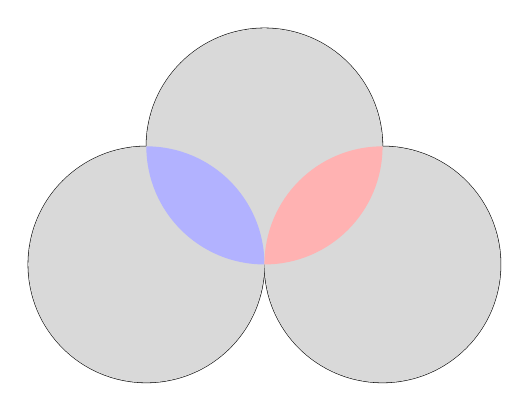
\begin{tikzpicture}[scale=1.5]

        % 定义三个圆的位置和大小
        \draw (0,0) circle (1cm) node[above left] {A};
        \draw (2,0) circle (1cm) node[above right] {B};
        \draw (1,1) circle (1cm) node[above] {C};

        % 填充颜色(可选)
        \fill[gray!30] (0,0) circle (1cm); % A 的独有部分
        \fill[gray!30] (2,0) circle (1cm); % B 的独有部分
        \fill[gray!30] (1,1) circle (1cm); % C 的独有部分

        % 填充 AC 重叠部分(A 和 C 的交集)
        \begin{scope}
            \clip (0,0) circle (1cm);
            \fill[blue!30] (1,1) circle (1cm);
        \end{scope}

        % 填充 BC 重叠部分(B 和 C 的交集)
        \begin{scope}
            \clip (2,0) circle (1cm);
            \fill[red!30] (1,1) circle (1cm);
        \end{scope}

        % 确保 AC 和 BC 重叠部分面积相等(通过对称性保证)
    \end{tikzpicture}
    \end{center}
    则只有一个事件发生的概率为
        $(\frac{1}{4} - \frac{1}{12})\times 2 + \frac{1}{4} 
        - 2\times \frac{1}{12} = \frac{5}{12}$
    \end{solution}
    
    % 例题1.3
    \item 设随机事件$A,B$满足$AB=\bar{A}\bar{B}$,且$0<P(A)<1$,$0<P(B)<1$,则$P(A|\bar{B})+P(B|\bar{A})=\_\_\_\_\_$
    
    \begin{solution}
    \color{blue}
    根据结论,有$A,B$互斥,则$P(A|\bar{B})=P(B|\bar{A})=1$
    \end{solution}

    \begin{corollary}
        若$AB=\bar{A}\bar{B}$,则$A,B$必然对立
        \begin{align*}
            &AB =\bar{A}\bar{B} \\
            &\iff AB\cup \bar{A}B =\bar{A}\bar{B}\cup \bar{A}B \\
            &\iff (A\cup \bar{A})B = \bar{A}(\bar{B}\cup B) \\
            &\iff B = \bar{A}
        \end{align*}
    \end{corollary}

    % 例题 1.4
    \item 设随机事件$A,B,C$两两独立,满足$ABC=\varnothing$,且$P(A)=P(B)=P(C)$,$A,B,C$至少有一个发生的概率为$\frac{9}{16}$,则$P(A)=$
    
    \begin{solution}
    \color{blue}
    由题意有$P(A\cup B\cup C) = \frac{9}{16}$,由加法公式与独立性有
    \begin{align*}
        P(A\cup B\cup C) 
        &= P(A) + P(B) + P(C) - P(A)P(B) \\
        &- P(A)P(C) - P(B)P(C) - P(A)P(B)P(C)
    \end{align*}
    由$P(A)=P(B)=P(C)$,上式化为$3P(A)-3P(A)^2 = \frac{9}{16}\implies P(A)=\frac{1}{4}\text{或}P(A)=\frac{3}{4}$,
    显然$P(A)\neq \frac{3}{4} > P(A\cup B\cup C)$,故$P(A)=\frac{1}{4}$
    \end{solution}
    
    % 例题 1.5
    \item 设$A,B$为随机事件,且$P(A)=\frac{2}{3}$,$P(B)=\frac{1}{2}$,则$P(A|B)+P(B|A)$的最大值为\_\_\_\_,最小值为\_\_\_\_.
    
    \begin{solution}
    关于概率的不等式基于如下事实,对于任意一个概率其值均位于$[0,1]$之间,事件AB的和事件不可能小于单独A,B发生概率之和,事件AB的积事件不可能大于
    任意一个事件单独发生的概率.
    \[
    P(A)+P(B) - 1<=P(AB) \leq \min{(P(A),P(B))}  \leq P(A) + P(B) \leq P(A\cup B) 
    \]
    \end{solution}
\end{enumerate}

\section{三大概型的计算}
\begin{remark}[三大概率模型]
    \begin{enumerate}
    \item 经典概型 -- 有限个等可能的样本点,\textbf{排列组合问题}
    \item 几何概型 -- 使用几何参数度量概率,比如说长度,面积,体积等
    \item 伯努利概型 -- 独立重复试验每次成功的概率为$p$,不成功的概率为($1-p$)
    \end{enumerate}
\end{remark}
\begin{enumerate}[label=\arabic*.,start=6]
    % 例题 1.6
    \item (2016,数三)设袋中有红、白、黑球各1个,从中\textbf{有放回地}取球,每次取1个,直到三种颜色的球都取到为止,则取球次数恰好为4的概率为
    
    \begin{solution}
    (古典概型) 
    \[\frac{\binom{3}{1}\binom{2}{1}\binom{3}{2}}{3^4}=\frac{2}{9}\]
    首先从3个颜色中选择一个为第四次抽的颜色,再从剩下两个颜色中选择一个为出现两次的颜色,在选择该颜色抽出的次序.
    \end{solution}
    % 例题 1.7
    \item 在区间$(0,a)$中随机地取两个数,则两数之积小于$\frac{a^2}{4}$的概率为
    
    \begin{solution}
    (几何概型)
    \[
    \frac{\frac{a}{4}\cdot a + \int_{\frac{a}{4}}^{a}\frac{a^2}{4x}dx}{a^2} = \frac{1}{4} + \frac{1}{2}\ln{2}
    \]
    \end{solution}
    % 例题 1.8
    \item 设独立重复的试验每次成功的概率为$p$,则第5次成功之前至多2次失败的概率为
    
    \begin{solution}
    失败零次--$p^5$,失败一次--$\binom{1}{5}p^4(1-p)p$,失败两次--$\binom{2}{6}p^4(1-p)^2p$ \\
    故第5次成功之前至多2次失败的概率为
    \[
    p^5 + \binom{1}{5}p^4(1-p)p + \binom{2}{6}p^4(1-p)^2p
    \]
    \end{solution}
\end{enumerate}

\section{三大概率公式的计算}
\begin{remark}
    三大概率公式
    \begin{enumerate}
    \item 条件概率公式\qquad $P(A\mid B)=\frac{P(AB)}{P(B)}$ \\
    推论 
    \begin{align*}
        P(AB) &= P(B)P(A\mid B) \\
        P(\prod_{i=1}^{n}A_i) &= P(A_1)P(A_2\mid A_1)P(A_3\mid A_1A_2) \ldots P(A_n\mid A_1,\ldots,A_{n-1})
    \end{align*}
    \item 全概率公式\qquad $P(A)=\sum_{i=1}^{n}P(AB_i)=\sum_{i=1}^{n}P(B_i)P(A\mid B_i)$
    \item 贝叶斯公式\qquad $P(B_j\mid A)=\frac{P(B_j)P(A\mid B_j)}{\displaystyle \sum_{i=1}^{n}P(B_i)P(A\mid B_i)}$
    \end{enumerate}
    若称$P(B_j)$为$B_j$的先验概率,称$P(B_j\mid A)$为$B_j$的后验概率.则贝叶斯公式专门用于计算后验概率的公式.
\end{remark}

\begin{enumerate}[label=\arabic*.,start=9]
    % 例题 1.9
    \item 设$A,B$为随机事件,且$P(A\cup B)=0.6$,$P(B|\bar{A})=0.2$,则$P(A)=\_\_\_\_$
    
    \begin{solution}
    \[P(A\cup B)=P(A) + P(B) - P(AB) = 0.6, P(B\mid\bar{A})=\frac{P(B)-P(AB)}{1-P(A)} = 0.2\]
    联立有
    \[\frac{0.6 - P(A)}{1 - P(A)} = 0.2\],则$P(A)=0.5$
    \end{solution}
    
    % 例题 1.10
    \item  (2018,数一)设随机事件$A$与$B$相互独立,$A$与$C$相互独立,满足$BC=\varnothing$,且
    \begin{align*}
        P(A)=P(B)=\frac{1}{2},\quad P(AC|AB\cup C)=\frac{1}{4},
    \end{align*}
    则$P(C)=$\_\_\_\_.
    
    \begin{solution}
    \begin{align*}
        P(AC|AB\cup C)
        &= \frac{P(AC)}{P(AB\cup C)} \\
        &=\frac{P(A)P(C)}{P(AB)+P(C)} \\
        &=\frac{\frac{1}{2}P(C)}{\frac{1}{4} + P(C)} = \frac{1}{4}
    \end{align*}
    则$P(C)=\frac{1}{4}$
    \end{solution}
    
    % 例题 1.11
    \item  (2003,数一)设甲、乙两箱装有同种产品,其中甲箱装有3件合格品和3件次品,乙箱装有3件合格品。从甲箱中任取3件产品放入乙箱,
    \begin{enumerate}[label=(\roman*)]
        \item[(1)] 求乙箱中次品件数$X$的数学期望;
        \item[(2)] 求从乙箱中任取一件产品是次品的概率.
    \end{enumerate}

\begin{solution}[用概率计算]
    \begin{enumerate}
    \item[(1)] 对于数字特征的题目,先求概率分布再说,由于$P(X=k)=\frac{C_{3}^{k}C_{3}^{3-k}}{C_{6}^{3}}$
    $$
    \begin{array}{c|c c c c}
    X  & 0 & 1 & 2 & 3 \\ \hline
    P(x)  &  \frac{1}{20}  &  \frac{9}{20}  &  \frac{9}{20}  &  \frac{1}{20}
    \end{array}
    $$
    则所求数学期望$EX=\frac{9}{20} + 2\times \frac{9}{20} + \frac{3}{20} = \frac{3}{2}$
    \item [(2)] 
    \begin{align*}
        P(A) &=\sum_{k=0}^{3}P(X=k)P(A\mid x=k)  \\
        &= \frac{1}{20} \times 0 + \frac{9}{20}\times\frac{1}{6} 
        + \frac{9}{20}\times\frac{2}{6} + \frac{1}{20}\times \frac{3}{6}  \\
        &= \frac{1}{4}
    \end{align*}
    \end{enumerate}
\end{solution}

\begin{solution}[使用超几何分布]
    \begin{enumerate}
    \item [(1)] $X\sim H(N, M, n), N = 6, M = 3, n = 3$, 则$EX=\frac{nM}{N}=\frac{3}{2}$
    \item [(2)]
    \begin{align*}
        P(A) &=\sum_{k=0}^{3}P(X=k)P(A\mid x=k) \\
        &= \sum_{k=0}^{3}P(X=k) \frac{k}{6} \\
        &= \frac{1}{6}\sum_{k=0}^{3}P(X=k)k \\
        &= \frac{1}{6}EX \\
        &= \frac{1}{4}
    \end{align*}
    \end{enumerate}
\end{solution}

\end{enumerate}

\section{事件独立的判定}

\begin{remark}[事件独立的充要条件]
\begin{align*}
        & P(AB) = P(A)P(B) \\
        & \iff P(A\mid B) = P(A) \\
        & \iff P(A\mid \bar{B}) = P(A) \iff P(A\mid B) = P(A\mid \bar{B}) \quad (0 < P(B) < 1) \\
        & \iff A \text{ 与 } \bar{B}, \text{ 或 } \bar{A} \text{ 与 } B, \text{ 或 } \bar{A} \text{ 与 } \bar{B} \text{ 相互独立} \\
        & \iff P(A\mid B) + P(\bar{A} \mid \bar{B}) = 1, \quad 0 < P(B) < 1
\end{align*}
\end{remark}

\begin{enumerate}[label=\arabic*.,start=12]
    % 例题 1.12
    \item  设$A,B$为随机事件,且$0<P(A)<1$,则 \\
        (A)\ 若$A\supset B$,则$A,B$一定不相互独立 \\
        (B)\ 若$B\supset A$,则$A,B$一定不相互独立 \\
        (C)\ 若$AB=\varnothing$,则$A,B$一定不相互独立 \\
        (D)\ 若$A=\bar{B}$,则$A,B$一定不相互独立
    
    \begin{solution}
    (A)(B)(C)考虑$\varnothing$则都不对\\
    (D)由于A不是必然事件,则$B$不是不可能事件,则$0<P(A)<1,0<P(B)<1$,根据下面的总结$A,B$一定不独立
    \end{solution}
    \begin{tcolorbox}[title=总结]
        (1)概率为0或1的事件与任意事件独立 \\
        特别的,不可能事件与必然事件与任意事件独立 \\
        (2)设$0<P(A)<1, 0<P(B)<1$, \\
        $A,B$互不相容,则$A,B$一定不独立 \\
        $A,B$独立,则$A,B$一定不互不相容
    \end{tcolorbox}
    % 例题 1.13
    \item  设$A,B,C$为随机事件,$A$与$B$相互独立,且$P(C)=0$,则$\bar{A},\bar{B},\bar{C}$
    \begin{choices}[2]
    \task 相互独立 
    \task 两两独立,但不一定相互独立
    \task 不一定两两独立 
    \task 一定不两两独立
    \end{choices}
    \begin{solution}
    由$P(C)=0$知$A,B,C$相互独立,则$\bar{A}\bar{B}\bar{C}$也相互独立.
    \end{solution}

\end{enumerate}
\begin{tcolorbox}[title=两两独立与相互独立]
    \begin{align*}
        \text{相互独立}\left\{\begin{matrix}
        \left.\begin{matrix}
        P(AB)=P(A)P(B) \\
        P(AC)=P(A)P(C) \\
        P(BC)=P(B)P(C)
        \end{matrix}\right\}& \text{两两独立} \\
        P(ABC)=P(A)P(B)P(C)
        \end{matrix}\right.
    \end{align*}
\end{tcolorbox}

\ifx\allfiles\undefined
\end{document}
\fi